\vspace{-10pt}
\section{GradCAM}\label{sec:approach}
A number of previous works have asserted that deeper representations in a CNN capture higher-level visual constructs~\cite{bengio2013representation,mahendran2016visualizing}.
Furthermore, convolutional layers naturally retain spatial information which is lost in fully-connected layers, so we can expect the last convolutional layers to have the best compromise between high-level semantics and detailed spatial information.
The neurons in these layers look for semantic class-specific information in the image (say object parts).
GradCAM uses the gradient information flowing into the last convolutional layer
of the CNN to assign importance values to each neuron for a particular decision of interest.
\rp{
    Although our technique is fairly general in that it can be used to explain
    activations in any layer of a deep network, in this work, we focus on explaining
    output layer decisions only.
}

As shown in \reffig{fig:approach}, in order to obtain the class-discriminative localization map GradCAM
$L_{\text{GradCAM}}^c$ $\in \mathbb{R}^{u \times v}$ of width $u$ and height $v$ for any class $c$,
we first compute the gradient
of the score for class $c$, $y^c$ \mac{(before the softmax)}, with respect to feature map
activations $A^k$ of a convolutional layer, \ie $\frac{\del y^c}{\del A^k}$.
These gradients flowing back are global-average-pooled~\footnote{\rpi{Empirically we found global-average-pooling to work better than global-max-pooling as can be found in the Appendix. }}
\ad{
    over the width and height dimensions (indexed by $i$ and $j$ respectively)}
to obtain the neuron importance weights $\alpha{}_{k}^c$:
\begin{center}
\begin{equation} \label{eq:alpha1}
    \alpha{}_{k}^c =
    \overbrace{
        \frac{1}{Z}\sum_{i}\sum_{j}
    }^{\text{global average pooling}}
    \hspace{-17pt}
    \underbrace{
        \vphantom{\sum_{i}\sum_{j}} \frac{\partial y^c}{\partial A_{ij}^{k}}
    }_{\text{gradients via backprop}}
\end{equation}
\end{center}
\rpi{During computation of $\alpha{}_{k}^c$ while backpropagating gradients with respect to activations, the exact computation amounts to successive matrix products of the weight matrices and the gradient with respect to activation functions till the final convolution layer that the gradients are being propagated to. }
Hence, this weight $\alpha{}_{k}^c$ represents a \emph{partial linearization} of the deep network downstream from A,
and captures the `importance' of feature map $k$ for a target class $c$. 

We perform a weighted combination of forward activation maps, and follow it by a ReLU to obtain,
\begin{center}
\begin{equation} \label{eq:gcam}
    L_{\text{GradCAM}}^{c} = ReLU \underbrace{\left(\sum_k \alpha{}_{k}^{c} A^{k}\right)}_{\text{linear combination}}
\end{equation}
\end{center}
Notice that this results in a coarse heatmap of the same size as the convolutional feature
maps ($14 \times 14$ in the case of last convolutional layers of VGG \cite{simonyan_arxiv14} and AlexNet \cite{krizhevsky_nips12} networks) \footnote{\rpi{We find that GradCAM maps become progressively worse as we move to earlier convolutional layers as they have smaller receptive fields and only focus on less semantic local features.}}.
\mac{We apply a ReLU to the linear combination of maps because we are only interested in the features that have a \emph{positive} influence on the class of interest, \ie
pixels whose intensity should be \emph{increased} in order to increase $y^c$.
Negative pixels are likely to belong to other categories in the image.
As expected, without this ReLU, localization maps sometimes highlight more than
just the desired class and perform worse at localization.}
Figures \hyperlink{page.2}{1c, 1f} and \hyperlink{page.2}{1i, 1l} show GradCAM visualizations for `tiger cat'
and `boxer (dog)' respectively. 
Ablation studies are available in ~\secref{sec:ablation}. 


\mac{
    In general, $y^c$ need not be the class score produced by an image classification
    CNN. It could be any differentiable activation including words from a caption or
    answer to a question.
}

\vspace{-10pt}
\subsection{GradCAM generalizes CAM}
\label{sec:generalization}
\ijcv{In this section, we \ad{discuss the connections between GradCAM and Class Activation Mapping (CAM)~\cite{zhou_cvpr16},
and formally  prove that GradCAM generalizes CAM} for a wide variety of CNN-based architectures.}
\noindent Recall that CAM produces a localization map for an image classification
CNN with a specific kind of architecture where global average pooled convolutional feature maps
are fed directly into softmax.
Specifically, let the penultimate layer produce $K$ feature maps,
$A^k \in \mathbb{R}^{u \times v}$, with each element indexed by $i,j$.
So $A_{ij}^k$ refers to the activation at location $(i,j)$ of the feature map $A^k$.
These feature maps are then spatially pooled using Global Average Pooling (GAP)
and linearly transformed to produce a score $Y^c$ for each class $c$,
\begin{center}
\begin{equation} \label{eq:scores}
    Y^c = \sum_{k}
	\hspace{-20pt}
    \underbrace{
        \vphantom{\frac{1}{Z}\sum_i \sum_j} w^c_k
    }_{\vspace{-3pt}
	\text{class feature weights}}
    \hspace{-27pt}
    \overbrace{
        \frac{1}{Z}\sum_i \sum_j
    }^{\text{global average pooling}}
    \hspace{-15pt}
    \underbrace{
        \vphantom{\frac{1}{Z}\sum_i \sum_j} A^k_{ij}
    }_{\vspace{-5pt}\text{feature map}}
\end{equation}
\end{center}




Let us define $F^k$ to be the global average pooled output,
\begin{center}
\begin{equation}\label{eq:cam_gap}
    F^{k} = \frac{1}{Z} \sum_{i} \sum_{j} A_{ij}^k
\end{equation}
\end{center}

CAM computes the final scores by,
\begin{center}
\begin{equation}\label{eq:cam_scores}
    Y^c = \sum_{k} w_{k}^c \cdot F^{k}
\end{equation}
\end{center}
where $w_{k}^c$ is the weight connecting the $k^{th}$ feature map with the $c^{th}$ class.
Taking the gradient of the score for class c ($Y^c$)  with respect to the feature map $F^k$ we get,
\begin{center}
\begin{equation}\label{eq:cam_grad}
    \frac{\partial Y^c}{\partial F^k} = \frac{\frac{\partial Y^c}{\partial A_{ij}^k}}{\frac{\partial F^k}{\partial A_{ij}^k}}
\end{equation}
\end{center}

Taking partial derivative of  \eqref{eq:cam_gap} \wrt $A_{ij}^k$, we can see that $\frac{\del F^k}{\del A^k_{ij}} = \frac{1}{Z}$. Substituting this in \eqref{eq:cam_grad}, we get,
\begin{center}
\begin{equation}
    \frac{\partial Y^c}{\partial F^k} = \frac{\partial Y^c}{\partial A_{ij}^k} \cdot Z\\
\end{equation}
\end{center}

From \eqref{eq:cam_scores} we get that, $ \frac{\partial Y^c}{\partial F^k} = w_{k}^c$. Hence,

\begin{center}
\begin{equation}\label{eq:cam_weights}
    w_{k}^c = Z \cdot \frac{\partial Y^c}{\partial A_{ij}^k}\\
\end{equation}
\end{center}

Summing both sides of \eqref{eq:cam_weights} over all pixels $(i,j)$,

\begin{center}
\begin{equation}
    \sum_i \sum_j w^c_k  = \sum_i \sum_j Z \cdot \frac{\del Y^c}{\del A^k_{ij} }
\end{equation}
\end{center}

Since $Z$ and $w^c_k$ do not depend on $(i,j)$, rewriting this as

\begin{center}
\begin{equation}
    Z w^c_k  = Z \sum_i \sum_j \frac{\del Y^c}{\del A^k_{ij}}
\end{equation}
\end{center}

Note that $Z$ is the number of pixels in the feature map (or $Z = \sum_i \sum_j \mathbf{1} $).
Thus, we can re-order terms and see that

\begin{center}
\begin{equation}
    w^c_k  = \sum_i \sum_j \frac{\del Y^c}{\del A^k_{ij} }\\
\end{equation}
\end{center}

Up to a proportionality constant ($1/Z$) that gets normalized-out during
visualization, the expression for $w^c_k$ is identical to $\alpha^c_k$ used by GradCAM \eqref{eq:alpha1}.
Thus, GradCAM is a strict generalization of CAM.
This generalization allows us to generate visual explanations from CNN-based
models that cascade convolutional layers with much more complex interactions,
such as those for image captioning and VQA (\refsec{sec:vqa}).

\vspace{-5pt}
\subsection{\cgb{}}
While GradCAM is class-discriminative and localizes relevant image regions,
it lacks the ability to highlight fine-grained details like pixel-space gradient
visualization methods (\gb{}~\cite{springenberg_arxiv14}, \dec{}~\cite{zeiler_eccv14}).
\ad{\gb{} visualizes gradients with respect to the image where
    negative gradients are suppressed when backpropagating through ReLU layers.
    Intuitively, this aims to capture pixels detected by neurons, not
    the ones that suppress neurons.}
See Figure \hyperlink{page.2}{1c}, where
GradCAM can easily localize the cat; however, it is unclear from the coarse
heatmap why the network predicts this particular instance as `tiger cat'.
In order to combine the best aspects of both, we fuse \gb{} and GradCAM visualizations
via element-wise multiplication
($L_{\text{GradCAM}}^c$ is first upsampled to the input image resolution using bilinear interpolation).
\figref{fig:approach} bottom-left illustrates this fusion.
This visualization is both high-resolution (when the class of interest is `tiger cat',
it identifies important `tiger cat' features like stripes, pointy ears and eyes) and
class-discriminative (it highlights the `tiger cat' but not the `boxer (dog)').
Replacing \gb{} with \dec{} gives similar results, but we found \dec{}
visualizations to have artifacts and \gb{} to be generally less noisy.

\subsection{Counterfactual Explanations}


Using a slight modification to GradCAM, we can obtain explanations
that highlight support for regions that would make the network change its prediction. 
As a consequence, removing concepts occurring in those regions would make the
model more confident about its prediction. 
We refer to this explanation modality as counterfactual explanations.

Specifically, we negate the gradient of $y^c$ (score for class $c$) with respect to feature maps $A$ of a convolutional layer.
Thus the importance weights $\alpha{}_{k}^{c}$ now become
\begin{center}
\begin{equation} \label{eq:alpha_neg}
    \alpha{}_{k}^c =
    \overbrace{
        \frac{1}{Z}\sum_{i}\sum_{j}
    }^{\text{global average pooling}}
    \hspace{-17pt}
    \underbrace{
        \vphantom{\sum_{i}\sum_{j}} -\frac{\partial y^c}{\partial A_{ij}^{k}}
    }_{\text{Negative gradients}}
\end{equation}
\end{center}
As in \eqref{eq:gcam}, we take a weighted sum of the forward activation maps, $A$, with weights $\alpha{}_{k}^c$, and follow it by a ReLU to obtain counterfactual explanations as shown in \reffig{fig:negexp}.

\begin{figure}[ht!]
    \centering \begin{subfigure}[t]{0.158\textwidth} \centering
        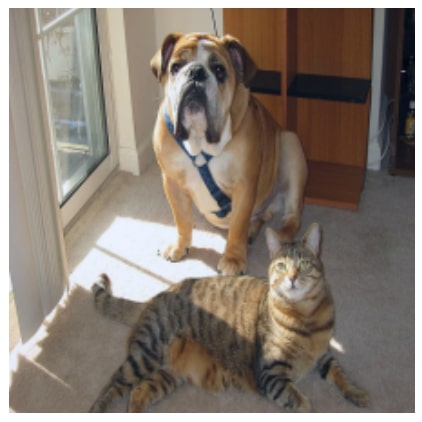
\includegraphics[width=\textwidth]{figures/teaser/original.jpg}
        \caption{\scriptsize{Original Image}}
	\end{subfigure}
	\begin{subfigure}[t]{0.158\textwidth}
        \centering
        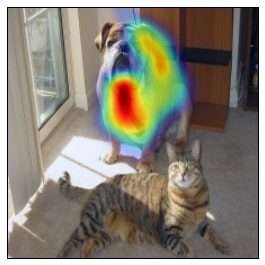
\includegraphics[width=\textwidth]{figures/cat_neg_exp.jpg}
        \caption{\scriptsize{Cat Counterfactual exp}}
		\label{fig:neg_exp_cat}
	\end{subfigure}
    \centering
	\begin{subfigure}[t]{0.158\textwidth}
        \centering
        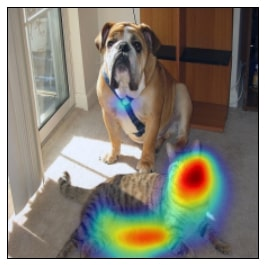
\includegraphics[width=\textwidth]{figures/dog_neg_exp.jpg}
        \caption{\ijcv{\scriptsize{\hspace{-1pt}Dog Counterfactual exp}}}%
		\label{fig:neg_exp_dog}
	\end{subfigure}
    \vspace{10pt}
    \caption{Counterfactual Explanations with GradCAM}
    \label{fig:negexp}
\end{figure}






